\section{Related work}
\subsection{Internet of things}
Cluster of European research projects \cite{Gubbi2013}  regarding the Internet of Things:
\begin{quote}
    'Things' are active participants in buissness, information and social processes where they are enabled to interact and communicate aming themselves and with the enviorment by exhchanging data and information sensed about the envoirment while reacting autonomously to real/physical world events and influencing it by runnign processes that trigger actions and create services with or without direct human intervention.
%Fix correct qoute on this!
\end{quote} 

Gubbi et. al. \cite{Gubbi2013} defines the Internet of Things as:
\begin{quote}
    Interconnection of sensing and actuating devices providing the ability to share inforamtion across platforms through a unified framework, developing a common operating picture for enabling innovative applications. 
    This is achieved by seamless large scale sensing, data analytics and information representation using cutting egde ubiquitous sensing and cloud computing.
\end{quote}

\subsection{Industry 4.0}
%Industry 4.0 definition.
Lasi \cite{Lasi2014}  argues that the term industry 4.0 was coined beforehand as a planned fourth industruial revolution.
The use of internet of things devices, IoT-devices from now on, and cyber physical systems, CPS from now on is what defines the fourth industrial revolution Vadiya means \cite{Vaidya2018}.
See figure x for a short historic overview of previous industrial revolutions. 
\begin{figure}
    \centering
    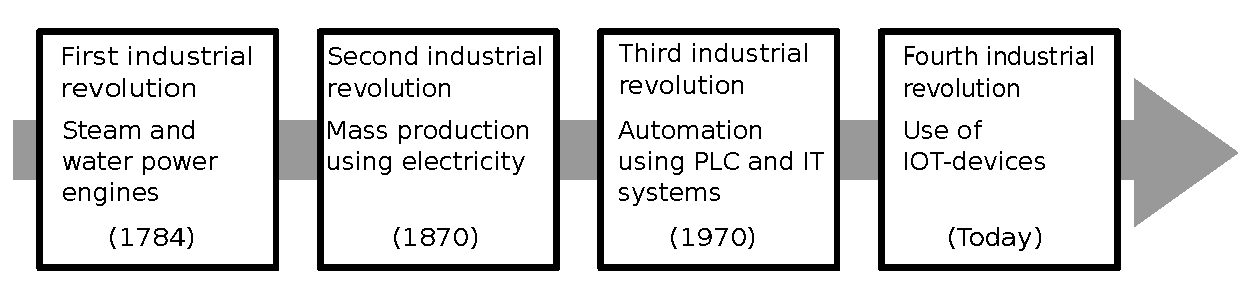
\includegraphics[width=\textwidth]{Pictures/Industrial_revolution.pdf} 
    \caption{Historic overview of previous industrial revolutions}
    \label{Indutrial revolutions}
\end{figure}

According to Vadiya \cite{Vaidya2018} industry 4.0 promotes the connection of sensors and devices both to the internet and to other sensors or devices.

%Intelligent  sensors.
Hozdić \cite{Hozdic2015} states that a sensor is a device capable of providing an appropriate output in response to a measured value.
One key feature of intelligent sensor is that in order to increase the level of information proeccesing it processes the information at a logical level Hozdić \cite{Hozdic2015} argues.
A Intelligent sensor  is capable of executing actions based on the measured value in contrast to regular sensors, making them easier to set up and use means Hozdić \cite{Hozdic2015}.

%Cyber Physical Systems (CPS).
Hozdić defines cyber physical system, CPS, as a new generation of system that integrate both physical and computer abilities. \cite{Hozdic2015}
A cyber physical system consists of two parts, one cybernetic and one physical.
The cybernetic part of the system can be viewed as a summation of logic and sensor units while the physical part of the system can be viewed as a summation of the accuator units Hozdić adds. \cite{Hozdic2015}
Xu et. al. states that cyber physical systems is a key part of Industry 4.0. In contrast to the simple embedded systems of today will be exceeded due to advances in CPS that enables enhanced capability, scalability, adaptibility, resilency, safety, usability and secruity.  \cite{Xu2018}
Hozdić argues that it is the CPS abilities to share and recieve information from intelligent sensors that connect to digital networks is what enables and form an internet of things. \cite{Hozdic2015}
 
\subsection{Arrowhead framework}
%Local cloud.
A local cloud is defined as a self contained network with at least the thrre mandatory systems deployed, more on those in a later paragragh. 
Delsing et.al. also argues that except the three mandatory core systems running a local cloud also needs at least one application system deployed \cite{Delsing2017}.

%Service and systems.
Two terms have to be introduced in order to further understand what the Eclipse Arrowhead framework aims to accomplish, services and systems.
Delsing et. al. defines a system as what is providing or consuming a service. \cite{Delsing2017} 
Furthermore a service is defined as what is used to convey information between a provider and a consumer Delsing et. al. argues \cite{Delsing2017}

%Mandatory core systems.
The Eclipse Arrowhead framework, Arrowhead from now on, consists of three mandatory core systems according to Delsing et. al. \cite{Delsing2017}
To fully operate a local cloud as defined in the previous section it must according to Delsing \cite{Delsing2017} contain:
\begin{itemize}
    \item Service registry system.
    \item Authorization system. 
    \item Orchestration system.
\end{itemize}
%Service registry system.
The service registry system is responsibly for enabling discovery and registring services Delsing et. al. \cite{Delsing2017} states. 
According to the Eclipse Arrowhead projects own github page \cite{Github2021} the service registry system provides the database which stores the offered services in the local cloud.
The github page also states the three main objectives of the service registry system are:
\begin{itemize}
    \item To allow application system to register available services to the database. 
    \item Remove or update available services from the database.
    \item Allow application system to use the lookup functionality of the registry.
\end{itemize}
%Authorization system.
The Authorization system is contains two databases for keeping track on which system can consume services from which other system, depending on whether or not the Application system are in the same cloud or not according the projects github page \cite{Github2021}
The github documentation also states that if the authorization happens within the same cloud it is called intra-cloud authorization and if it happens accross two local clouds it is called inter-cloud authorization. \cite{Github2021}

%Orchestrator system.
The Orchestration system is responsible for pairing and finding service providers and consumer Delsing et. al. declares. \cite{Delsing2017} 
Delsing et. al. continues to state that the orchestrator also stores the orchestration requirments and the resulting orchestration rules. \cite{Delsing2017} 
The projects documentation argues that the main objective of the orcherator system is to find an appropriate provider for the requesting consumer system. \cite{Github2021}
The documentation also states that there are two types of orchestration, store orchestration and dynamic orchestration.
Store orchestration uses the database orchestration store to find predefined orchestration rules.
Dynamic orchestration on the other hand searches the entire local cloud, or even other clouds, in order to find mathing provider. \cite{Github2021}

\subsection{Security}
%Introduction.
Meneghello et. al. argues that the increasing number of IoT-devices and the pervasive nature of new smart home or healthcare devices can pose a real threat to the users integritiy.
Sensitive information Meneghello et. al. defines as video recording of the users home, the users location, access to buildings, health monitoring and industrial processes. \cite{Meneghello2019}

%Secruity challenges.
Meneghello et. al. states the the secruity requirments of an IoT-system can be divied in to three different operational levels, namely the information, access and functional level. \cite{Meneghello2019}
The information level should garantee that the integrity, anonymity, confiidentiality and privacy of the system is preserved. 
Meaning that messages should not be altered with during transmission, the identity of the data source and the clients private information remains hidden and that data cannot be read by third parties Meneghello et. al. argues \cite{Meneghello2019} 
The access level provides a guarantee that only legitimate users are allowed access to the network and the devices associatied with that network. 
It also gaurantees that users within the network only uses resources they are allowed to use Meneghello et. al. states. \cite{Meneghello2019}
The functional level should guarantee the continued functionality of a network even in the case of malfunction or a malicous attack.

%Pricacy.
Zhang also argues that privacy is a big concern with IoT devices and suggests two solutions data collection policy and data anonymization. \cite{Zhang2014}
A policy for that describes how the data is collected from the devices would restrict the flow of data, therefore ensuring privacy preservation can be ensured Zhang states. \cite{Zhang2014}
Data anonymization means that the private information sent by the IoT devices is either encrypted or that the relation of the data and its owner is concealed according to Zhang. \cite{Zhang2014}

%Encryption.
Meneghello et. al. argues that on of the main aspect to security within IoT is to ensure that the data sent is the data recieved and that the data has not been tampered with or read during transmission.
The most important operation to guarantee that is the use of encryption, which converts the message sent in plain text to an encrypted message only readable with a decryption key Meneghello et. al. states. \cite{Meneghello2019}
Meneghello et. al. states that there are two mechanisms for encryption, symetric and asymetric. 
Symetric encryption is when the same key is used for encryption and decryption, so it has to be shared to both the sender and reciever.
Assymetric encryption on the other hand only shares the public key and the sender and reciever has their own private keys Meneghello et. al. means.

%End-to-End encryption.
Hassija et. al. states the importance of end-to-end encryption and the challenges it poses for the IoT systems. 
End-to-end encryption is required to ensure the confiidentiality of the data, the application should not let anyone execept the intended recipient read the messages sent Hassija adds.\cite{Hassija2019}

%Authentification.
Noor, Meneghello and Zhang states the importance of authentification in IoT systems. \cite{Noor2019,Meneghello2019,Zhang2014} 
Noor adds that 60\% of all IoT systems uses authentification to grant acceess to the user.  
Zhang argues that public key cryptosystem provide more security compared to symetric encryption schemes, but has the draw back of having high computional overhead. \cite{Zhang2014} 

%Lightweight cryptography.
Noor argues that conventional cryptographic primativs are unsuitable for IoT devices due to thier lack of computional power and limited battery life and memory capacity.
With IoT devices lacking capabilites as background Noor, Meneghello and Zhang all aggree that a push for lightweight cryptography is required in order to ensure secruity of these devices. \cite{Noor2019,Meneghello2019,Zhang2014} 

\subsection{Communication} 
%MQTT
MQTT, Message Queue Telemetry Transport, is a lightweight messaging invented by IBM suitable for IoT Wukkadada means \cite{Wukkadada2018}. 
MQTT is a publish/subscribe protocol that requires a minimal footprint and bandwidth to connect an IoT device according to HIVEMQ. \cite{MQTT2021}
MQTT consists of a MQTT broker and MQTT clients, where the broker is responsible for sending messages between the sender and its recipients. 
A client on the other hand publishes a message to the broker that other clients can subscribe to HIVEMQ adds. \cite{MQTT2021}

%HTTP/HTTPS
HTTP, HyperText Transfer Protocol, is a request/response protocol consisting of clients and servers that communicate by exchanging indidivual messages. 
The clients are responsible for the requests and the servers are responsible for the response Mozilla developer network clarifies. \cite{HTTP2021} 
In contrast to the lightweight MQTT protocol with low overhead and bandwidth, HTTP can cause serious banwidth issues Wukkadada adds. \cite{Wukkadada2018}
The biggest benefits to using HTTP is that it supports the RESTful Web architecture and that it is a globally accepted web messaging standard Naik suggests. \cite{Naik2017} 

%Comparisson 
Naik argues that HTTP exceeds MQTT in message size, message overload, power consumption, resource requirment, bandwidth and latency. 
All things that are considered negative for a protocol. \cite{Naik2017}
On the other hand HTTP exceeds MQTT in interoperability, standardization, security and provisioning Naik adds. \cite{Naik2017}
All things that are considered positive for a protocol.
Shariatzadeh argues that that HTTP may be expansive for many IoT devices but it can be benfical due to the interoperability since it is developed for the web originally. \cite{Shariatzadeh2016}
Wukkadada also points out the lower power consumption of the MQTT protocol but adds that the more verbose HTTP protocol can be easier for developers to understand. \cite{Wukkadada2018}
Wukkada drives the point home of choosing MQTT for IoT devices. \cite{Wukkadada2018}
